%!TEX root=document.tex

\section{User Study}
\label{sec:user_study}

The previous section evaluated \SeeDB 
and our optimizations in terms of performance.
In this section, we assess the utility of \SeeDB's recommendations 
with real users.
First, we perform a study to validate our deviation-based distance metric.
We show that although simple, our deviation-based
metric can find visualizations users feel are interesting.
Second, we compare \SeeDB
to a manual charting tool without visualization recommendations.
We show that \SeeDB can enable users to find interesting visualizations
faster and can surface unexpected trends.
We also find that users overwhelmingly prefer \SeeDB over a manual charting 
tool.

\subsection{Validating Deviation-based Utility}
\label{sec:validating_metric}

\SeeDB uses deviation between the target and reference dataset as a measure
of interestingness of a visualization.

\stitle{Ground Truth.}
To validate deviation as a utility metric, we obtained ground truth data about
interestingness of visualizations and evaluated \SeeDB against it.
To obtain ground truth, we presented 5 data analysis experts with the Census 
dataset (Section \ref{sec:introduction}) the analysis task of
studying the effect of marital status on socio-economic indicators.
We presented experts with the full set of potential aggregate visualizations 
and asked them to classify each visualization as interesting or
not interesting {\em in the context of the task}.
Of the 48 visualizations, on average, experts classified 4.5 visualizations
(sd = 2.3) as being interesting for the task.
The small number indicates that of the entire set of potential visualizations, 
only a small fraction (\textasciitilde10\%) show interesting trends.
To obtain consensus on ground truth, we labeled
any visualization chosen by a majority of participants as 
interesting; the rest were not. 
This process identified 6 interesting and 42 uninteresting visualizations.
In addition to Figures~\ref{fig:interesting_viz} (interesting) and Figure 
\ref{fig:uninteresting_viz} (not interesting), Figure~\ref{fig:huhi} 
was labeled as interesting (according to a user: ``\ldots it
shows a big difference in earning for self-inc adults'') while 
Figure~\ref{fig:luli} was labeled as not interesting (notice the lack of deviation).
While some classifications can be explained using deviation, some cannot: 
Figure \ref{fig:huli} shows high deviation but was deemed to be uninteresting, 
while Figure \ref{fig:luhi} shows small 
deviation but was deemed to be interesting (``\ldots hours-per-week seems like a 
measure worth exploring''). 

% Figure \ref{fig:gt_examples} shows ground truth for four other visualizations: 
% Figure \ref{fig:huhi} shows another visualization that was chosen as interesting by 4 of 5 
% participants.
% According to participants, this visualization was interesting because ``\ldots it
% showed a big difference in earning for self-inc adults'' and indicated a trend to 
% be examined further.
% Figure \ref{fig:luli} in contrast shows a visualization that participants
% did not select as relevant.
% Notice that the two distributions in this chart do not show significant difference. 
% However, this is not to say that deviation was the only factor relevant for interestingness.
% Figure \ref{fig:huli}, for example, shows a visualization that in fact has high deviation, but was 
% not classified as interesting by any participants.
% Similarly, Figure \ref{fig:luhi} shows a visualization that shows less deviation but was 
% classified as interesting by 2 participants because the .

% The gold standard for evaluating a recommendation system is to obtain ground 
% truth about user preferences about
% various (ideally all) items and examine whether the system's recommendations 
% can correctly classify each item\cite{??}.
% We adopt the same evaluation strategy.
% For the census dataset and associated analytical task (discussed in Section 
% \ref{sec:introduction}), we obtain ground truth about the interesting-ness of 
% each potential visualizations of the dataset.
% We then evaluate whether \SeeDB can correctly classify visualizations as
% interesting or not interesting.

% \stitle{Obtaining Ground Truth}.
% To obtain ground truth, we recruited 5 participants with significant data analysis 
% experience (3 female, 2 male).
% We presented each participant with the Census dataset and the task of finding visualizations
% that showed interesting trends related to marital status (Section \ref{sec:introduction}).
% Participants were presented with the entire set of aggregate visualizations \mpv{how many}
% for this dataset and asked to classify visualizations as being interesting or 
% not-interesting for the task.
% Participants were also asked to explain verbally why they thought a visualization
% was interesting.
% We capped the study at 10 minutes.

\begin{figure}[t]
	\centering
	\begin{subfigure}{0.45\linewidth}
		{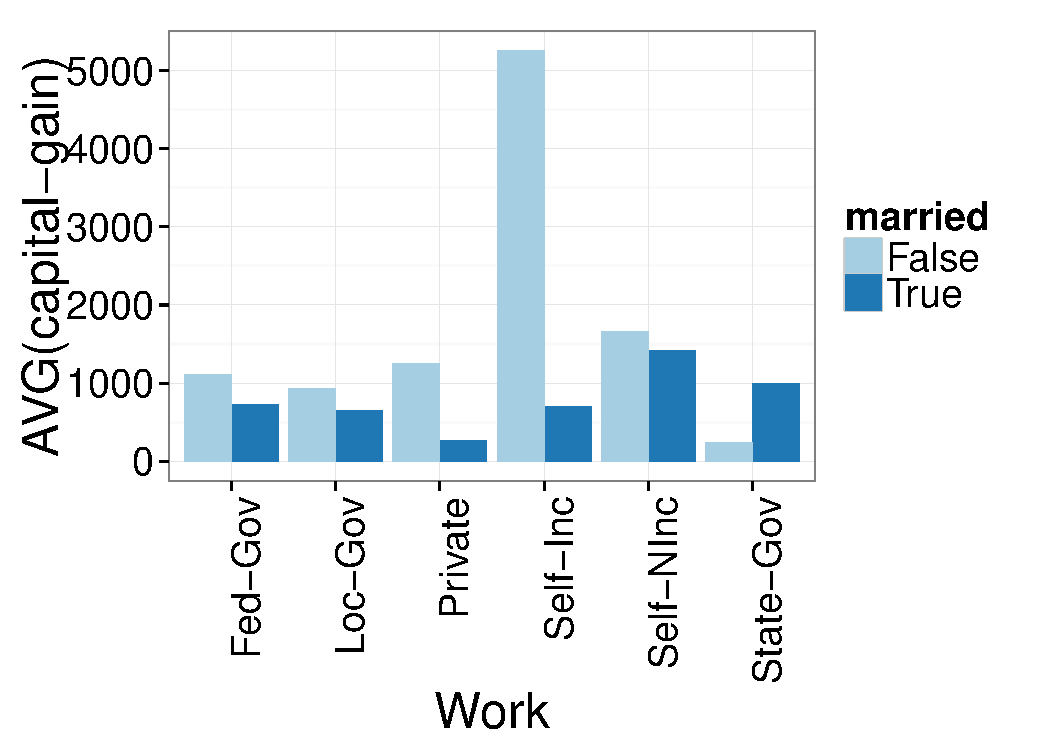
\includegraphics[width=4cm, trim=0 0 3cm 0, clip=true] {Images/HUHI_work_avg_cap_gain.pdf}}
		\caption{High deviation, interesting}
		\label{fig:huhi}  
	\end{subfigure}
	\begin{subfigure}{0.54\linewidth}
		{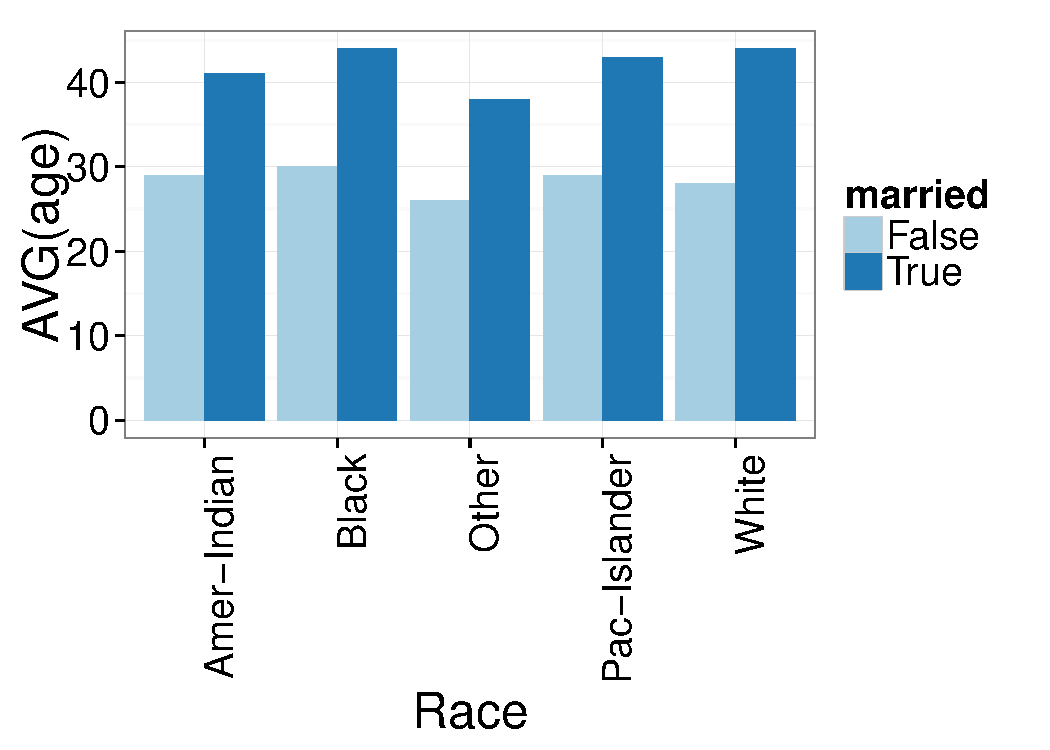
\includegraphics[width=4.5cm] {Images/LULI_race_avg_age.pdf}}
		\caption{Low deviation, not interesting}
		\label{fig:luli}
	\end{subfigure}
	\begin{subfigure}{0.45\linewidth}
		{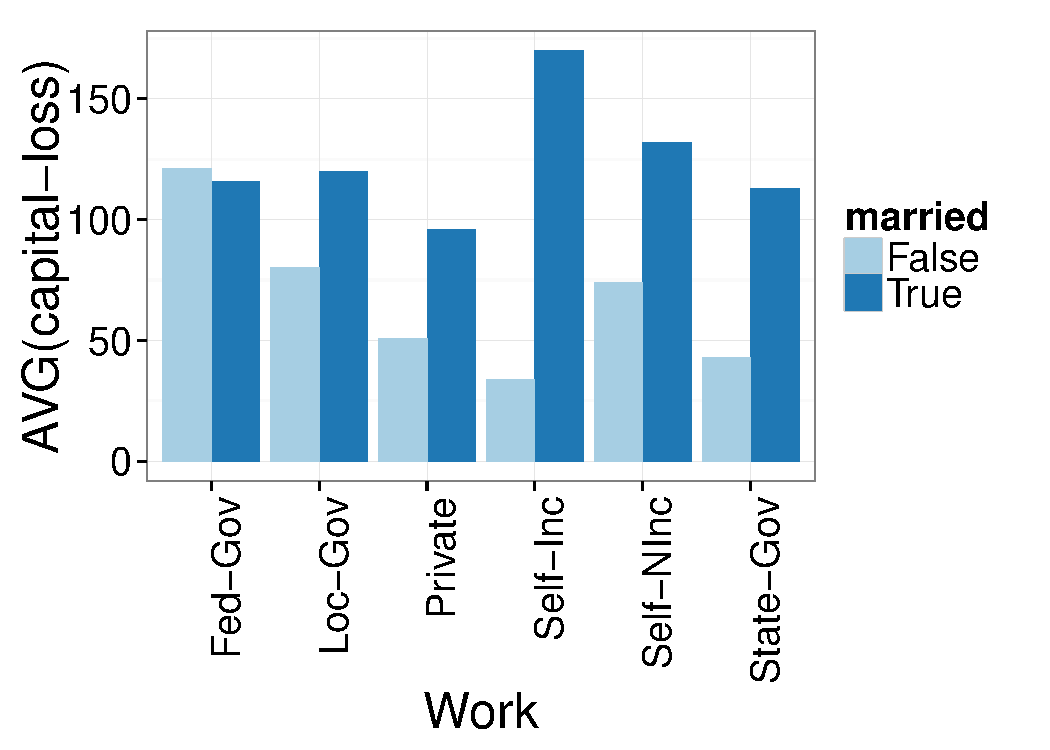
\includegraphics[width=4cm, trim=0 0 3cm 0, clip=true] {Images/HULI_work_avg_cap_loss.pdf}}
		\caption{High deviation, not interesting}
		\label{fig:huli}  
	\end{subfigure}
	\begin{subfigure}{0.54\linewidth}
		{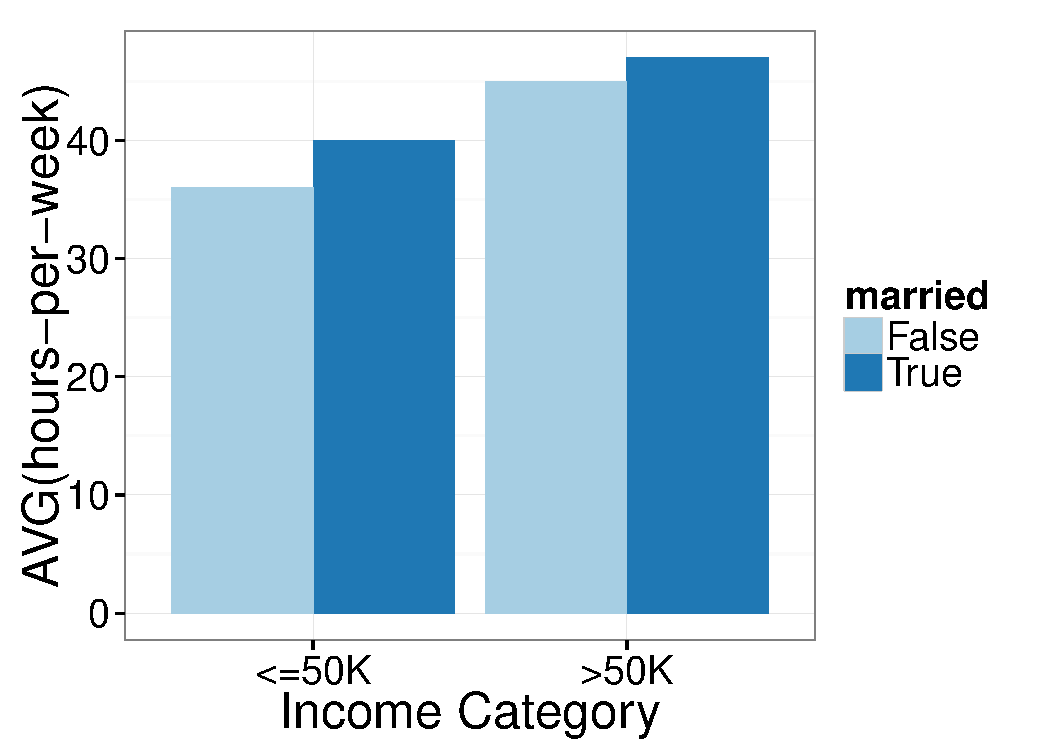
\includegraphics[width=4.5cm] {Images/LUHI_inc_avg_hours.pdf}}
		\caption{Low deviation, interesting}
		\label{fig:luhi}
	\end{subfigure}
	\vspace{-10pt}
	\caption{Examples of ground truth for visualizations}
	\vspace{-10pt}
	\label{fig:gt_examples}
\end{figure} 


% Figure \ref{fig:interesting_viz} in Section \ref{sec:introduction} (showing variation in
% average capital gain across sex for the single and married adults) was a visualization 
% classified as interesting by 4 or 5 participants. 
% In contrast, Figure \ref{fig:uninteresting_viz} was a visualization unanimously classified
% as uninteresting.

% Once we obtained ground truth, we evaluated whether \SeeDB could correctly
% classify visualizations with respect to ground truth.
% In all, participants selected 23 unique visualizations as being interesting.
% To obtain a consensus on ground truth, we used a simple voting system.
% Any visualization that was chosen by majority of participants (3 or more)
% was considered to be interesting; the rest were not.
% Of the 23 unique visualizations classified as interesting, majority of participants 
% agreed on 6 visualizations as being interesting.
% Observe that while there are subjective differences in the criteria for interesting-ness,
% it is possible to distill general criteria for interesting-ness of visualizations.

\begin{figure}[t]
	\centering
	\begin{subfigure}{0.32\linewidth}
		{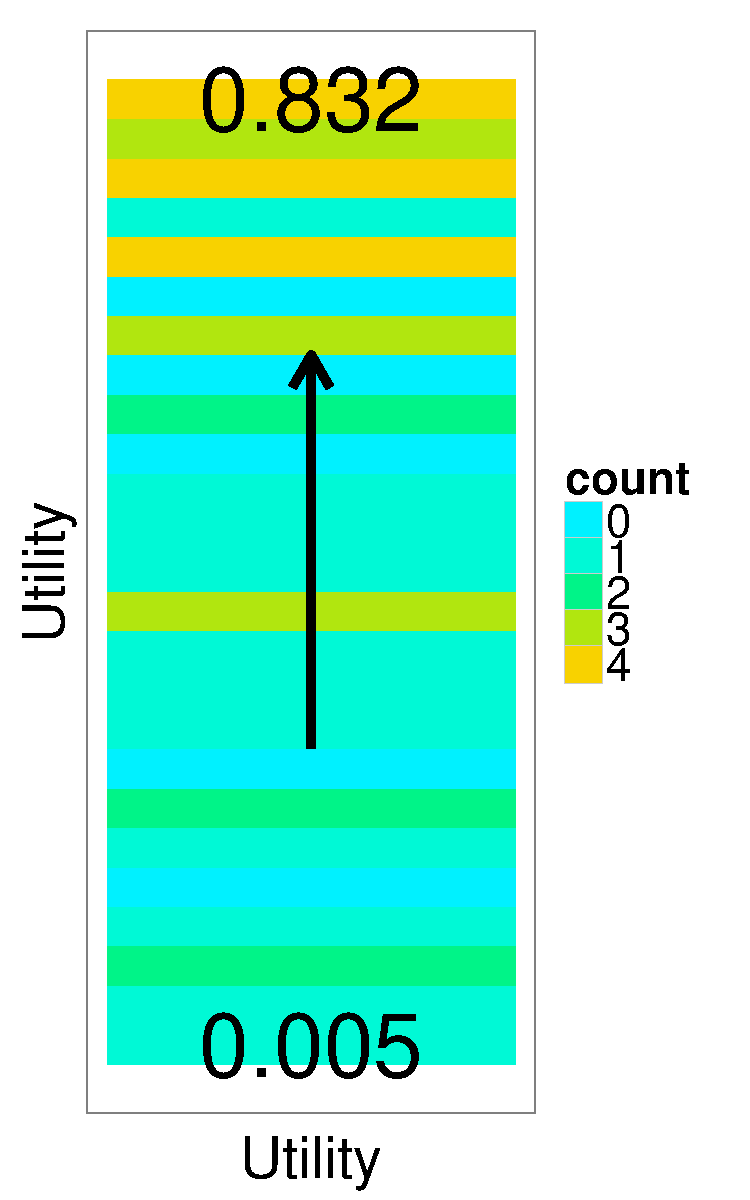
\includegraphics[trim={0 1.3cm 0 0}, clip, width=2.5cm]{Images/census_gt_distribution.pdf}}
		\caption{Utility Distribution}
		\label{fig:gt_dist}
	\end{subfigure}
	\begin{subfigure}{0.65\linewidth}
		\centering 
		{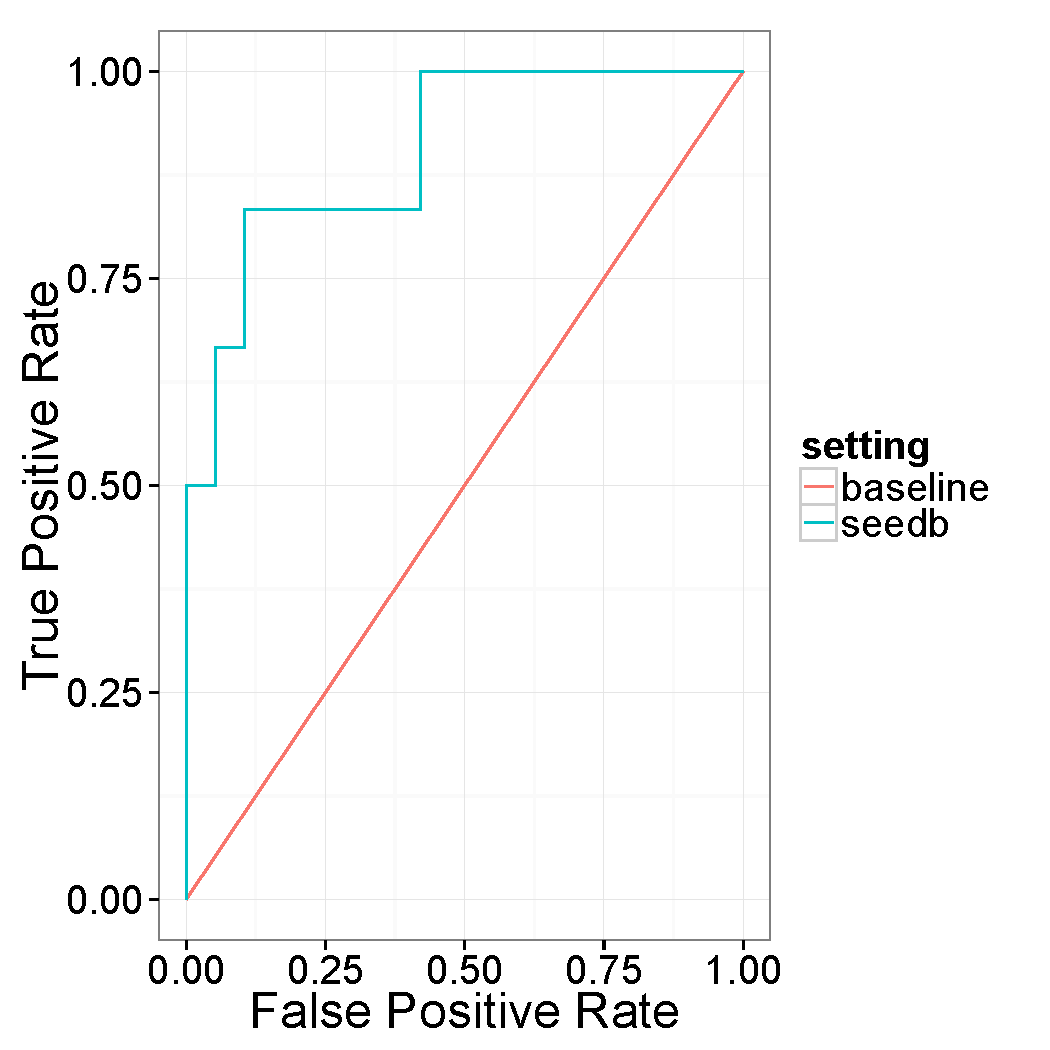
\includegraphics[width=4cm] {Images/seedb_roc.pdf}} 
		\caption{ROC of SeeDB (AUROC = 0.903)}
		\label{fig:roc}
	\end{subfigure}
	\vspace{-10pt}
	\caption{Performance of Deviation metric for Census data}
	\vspace{-20pt}
	\label{fig:census_gt}
\end{figure}

\stitle{Efficacy of Deviation-based Metric}.
Figure \ref{fig:gt_dist} shows a heatmap of the number of times a
visualization was classified as interesting 
({\em yellow} = popular, {\em blue} = not popular), sorted
in {\em descending order} of our utility metric.
We notice that the majority of yellow bands fall at the top of the
heatmap, indicating, qualitatively, that popular visualizations have higher utility.
To evaluate the accuracy of \SeeDB's recommendations over the Census data, 
we ran \SeeDB for the study task, varying $k$ between 0 \ldots 48, and measured
the agreement between \SeeDB recommendations and ground truth.
As is common in data mining, 
we computed the ``receiver operating curve'' or ROC curve for \SeeDB, 
Figure \ref{fig:roc}, depicting 
the relationship between the true positive rate (TPR) on the 
x-axis and false positive rate (FPR) on the y-axis for different values of a
parameter ($k$ in this case). 
TPR is the number of interesting visualizations returned as a fraction of the 
total number of interesting visualizations, 
while FPR is the fraction of recommendations
that were incorrectly returned as interesting, as a fraction of the number
of interesting visualizations returned. 
ROC curves for highly accurate classifiers are skewed towards the upper left
corner of the graph. The red line indicates the random baseline (every example
is classified randomly).
As can be seen in the figure, \SeeDB performs significantly better than the baseline.
For example, for $k$=3, all 3 visualizations recommended by \SeeDB are interesting,
giving TPR = 0.5 and FPR = 0; for $k$=5, 
four of the 5 recommended visualizations are interesting, 
giving TPR = 4/6 = 0.667 and FPR = 0.05. 
The area under ROC (AUROC) for \SeeDB---the typical measure of 
classifier quality---is 0.903.
This indicates that the accuracy of \SeeDB recommendations is very high.\footnote{\small AUROC's 
above 0.8 are considered very good, while those above 0.9 are
excellent}
%\mpv{add points on chart for k=3, 5}

While ROC curves on different datasets and tasks will vary,
this user study shows that \SeeDB recommendations have high quality
and coverage,
despite focusing on a simple deviation-based utility metric.
We expect that taking into account other aspects (apart from deviation),
would improve \SeeDB's recommendations even more.

% We varied the number of visualizations $k$ recommended by \SeeDB between 0 and
% max \mpv{fill in max}.
% For each value of $k$ we computed the number of true positives (\SeeDB recommended
% visualizations that were classified as ``interesting'' by majority), false
% positives, true negatives and false negatives.
% The true positive rate (recall) and false positive rate for \SeeDB are shown 
% in the `receiver operating curve'' (ROC)\cite{} in Figure \ref{fig:roc}.
% As expected, we observe that as $k$ increases, the true positive rate (TPR)
% increases (or stays constant), but false positive rate (FPR) also increases as 
% more visualizations are incorrectly classified as interesting.
% Clearly, \SeeDB performs significantly better than the baseline algorithm which 
% classifies every visualization as interesting with 50\% probability.
% For example, for $k$ = 3, TPR = 0.5 and FPR = 0;
% i.e., for $k$ = 3, all 3 visualizations recommended by \SeeDB are in fact interesting.
% However, \SeeDB recovers only 3 of the 6 visualizations.
% Likewise, for $k$ = 5, 4 of 5 of the recommended visualizations are interesting, giving
% TPR = 0.667 and FPR = 0.05.
% Finally, for $k$=14, \SeeDB recommends all 6 interesting visualizations, giving a 
% TPR of 1 but having an FPR of 0.421.
% The standard metric for computing quality of a recommender is to
% compute AUROC or area under the ROC curve.
% AUROC for \SeeDB in \ref{fig:roc} is 0.903.
% AUROC values above 0.8 are indicative of
% high quality of recommendations \cite{}, demonstrating that \SeeDB performs very well in
% making recommendations.

% While ROC curves for \SeeDB will vary with dataset and query, the above analysis, both
% qualitatively and via ROC, indicates that our deviation-based metric can in fact identify
% interesting visualizations with high accuracy.
% Although there are many other factors that determine interesting-ness, deviation seems
% to capture a significant part of the metric. 

% Now that we have validated our deviation-based metric, we examine how \SeeDB, a visualization tool
% with deviation-based recommendations, compares to a manual chart construction tool in performing
% visual analysis.

\subsection{{\large \SeeDB} vs. Manual Visualization Tool}
\label{sec:seedb_vs_manual}

%The motivation behind \SeeDB is to build a tool that can support fast
%visual analysis by automatically recommending interesting visualizations.
In this section, we describe results from a controlled user study comparing 
\SeeDB to a manual visualization tool for performing visual analysis. 
We hypothesized that: (i) when using \SeeDB, analysts would find interesting 
visualizations {\em faster} than when using the manual tool, (ii) analysts
would find {\it more} interesting visualizations when using \SeeDB vs. the 
manual tool, and (iii) analysts would {\em prefer} using \SeeDB to a manual tool.

% Next, we assess the efficacy of \SeeDB in enabling fast visual analysis.
% Towards this, we 
% To assess the efficacy of \SeeDB in enabling faster visual analysis,
% we conducted a user study where participants performed visual analysis
% using both \SeeDB and a manual chart construction tool.
% We hypothesized that: (i) When using \SeeDB, participants would find 
% interesting visualizations {\em faster} than when using manual chart
% construction, (ii) Participants would find more interesting visualizations
% when using \SeeDB vs. when using manual chart construction, (iii) 
% Participants would prefer using a tool with recommendations vs. a manual
% construction tool.

\stitle{Participants and Datasets}. We recruited 16 participants (5 female, 11
 male) all graduate students with prior data analysis experience and visualization
 experience (e.g. R, matplotlib or Excel).
 None of the participants had previously worked with the study datasets.

 Our study used the Housing and Movies datasets from 
 Table \ref{tab:datasets}.
 These  datasets were chosen because they were easy to understand and 
  comparable in size and number of potential visualizations.
 
\stitle{Study Protocol}.
Our study used a 2 (visualization tool) X 2 (dataset) within-subjects design.
The visualizations tools used were \SeeDB and {\em MANUAL}, a manual chart
construction-only version of \SeeDB (i.e., \SeeDB with the recommendations bar, 
component ``D'' in Figure \ref{fig:frontend1}, removed).
Using the same underlying tool in both modes allowed us to control for
tool functionality and user interface.
We used a within-subjects design to compensate for per-participant differences 
in data analysis expertise, and used counterbalancing to remove any effects 
related to order and the test dataset.

Our study began with a short tutorial on the two study tools.
Following the tutorial, participants were asked to perform two visual analysis 
tasks, one with \SeeDB in each mode.
For each mode, we introduced participants to the test dataset
and the analytical prompt using written instructions.
Each analytical task asked participants to use the specified tool to find 
visualizations supporting or disproving a specific hypothesis.
Participants were asked to use the bookmark button (in component ``C'' in Figure 
\ref{fig:frontend1}) to flag any visualizations they deemed interesting in
context of the task.
Participants were also encouraged to think aloud during the study.
Since the analytical tasks were open-ended, we capped each analysis session at 8 minutes.
Participants filled out a tool-specific survey at the end of each task and
an exit survey at the end of the study.
Most survey questions were answered on a 5-point Likert scale.
The study lasted \textasciitilde 45 minutes and participants were compensated 
 with a \$15 gift card.
All studies were conducted in a lab setting using Google Chrome on a 15-inch 
Macbook Pro.

\stitle{Methods and Metrics}.
Over the course of each study session, we collected data by three means: interaction logs 
from each tool, responses to surveys, and exit interview notes.
The interaction logs capture the number of visualizations
constructed, the number of visualizations bookmarked, bookmark rate, and interaction traces.
\SeeDB and MANUAL both support the construction of different types of charts such as bar 
charts, scatterplots etc.
Since \SeeDB can only recommend aggregate visualizations shown as bar charts,
we report results for aggregate visualizations.
We evaluate statistical significance of our results using paired t-tests and ANOVA,
and supplement interaction analysis with qualitative observations.


% Since users were asked to bookmark visualizations they found to be relevant to the task,
% bookmarking behavior from tool interaction logs provides a rich source
% of information about the analytical process.
% Specifically, we study a number of metrics including: (i) number of bookmarks ($num\_bookmarks$), 
% (ii) total number of visualizations viewed ($total\_viz$), 
% (iii) bookmarking rate ($bookmark\_rate$) defined as $num\_bookmarks$/$total\_viz$, and 
% (iv) the time between consecutive bookmarks ($bookmark\_time$).
% \SeeDB and MANUAL support construction of two kinds of charts: aggregate visualizations and 
% scatterplots (to replicate real visual analysis).
% Since \SeeDB can only recommend aggregate visualizations, we also analyze the above
% metrics for aggregate visualization only.
% We supplement bookmark analysis with qualitative data from surveys and study notes.
% We evaluate statistical signifance of our results using paired t-tests and ANOVAs.

\stitle{Results}.
Over the course of our study, participants built over 220 visualizations 
and bookmarked 70 visualizations (32\% bookmark rate).
We next describe our key findings and observations.

\stitle{1. \SeeDB enables fast visual analysis}.
Table \ref{tab:agg_bookmarks} shows an overview of the bookmarking behavior for each tool
focusing on total number of visualizations generated, number of bookmarks and bookmarking rate.
First, we observe that the total number of (aggregate) visualizations created in the \SeeDB
condition is higher than that for MANUAL. 
While not statistically significant, this difference suggests that analysts are exposed to more
{\em views} of the data with \SeeDB than MANUAL, possibly aiding in a more thorough exploration of
the data.
Next, we find that the number of aggregate visualizations bookmarked in \SeeDB is much higher (3X more)
than that for MANUAL.
In fact, the two-factor analysis of variance shows a significant effect of tool on the number of bookmarks,
F(1,1) = 18.609, p < 0.001. 
We find no significant effect of dataset, F(1, 1) = 4.16. p > 0.05, or
significant interaction between tool and dataset.
While this result indicates that analysts bookmark more visualizations in \SeeDB, we note that the number of 
bookmarks for a tool may be affected by the total number of visualizations built with the tool.
Therefore, to account for variance in the total number of visualizations, we also examine $bookmark\_rate$
for the two tools defined as the fraction of
created visualizations that are bookmarked ($\frac{num\_bookmarks}{total\_viz}$).
We find, once again, that the $bookmark\_rate$ for \SeeDB (0.42) is 3X larger than the $bookmark\_rate$ for 
MANUAL (0.14).
The two-factor analysis of variance shows a significant effect of tool on bookmark rate, F(1,1) = 10.034, p < 0.01.
As before, we find no significant effect of dataset on bookmark rate, F(1, 1) = 3.125. p > 0.05, or
significant interaction between tool and dataset.
Together the two results above indicate that there is a {\bf significant effect of tool on both the number of bookmarks as well as the
bookmark rate}.
\SeeDB-recommended visualizations are 3 times more likely to be interesting compared
to manually constructed visualizations.
%In other words, analysts are 3X more likely to arrive at interesting visualizations
%when using \SeeDB vs. MANUAL:
%\SeeDB can thus allow analysts to find analyze data faster. 
%\mpv{Remove? Finally, we note that the statistical results regarding faster analysis are supported by anecdotal evidence 
%and survey data from study participants.
Finally, 87\% of participants indicated that \SeeDB recommendations sped up their visual analysis, many alluding
to the ability of \SeeDB to ``\ldots quickly deciding what correlations are relevant'' and 
``[analyze]...a new dataset quickly''.


% Moreover, we once again find this difference in $bookmark\_rate$ is statistically significant
% within subjects as well as across subjects ({\em Paired t-test, t = -2.5599, df = 8, p-value = 0.03365}).
% This implies that {\bf a \SeeDB-recommended visualization is 3 times more likely to be
% interesting compared to a manually constructed aggregate visualization}.
% In other words, users are 3X more likely to arrive at interesting visualizations when using
% \SeeDB vs. MANUAL; i.e., \SeeDB can enable users to find interesting insights faster.
% Results of a 2-way ANOVA also indicate that \SeeDB has a significant impact on 
% aggregate bookmark rate ({\em df = 1, sum sq = 0.3681, mean sq = 0.3681, F value = 10.034, p = 0.00685}). 
% (We find that choice of dataset does not affect bookmark rate, and there are no interaction or order effects.)

% We also find that, on average, the $bookmark\_time$ for \SeeDB (92.91 $\pm$ 49.26) is twelve seconds 
% shorter than that for MANUAL (105.02 $\pm$ 58.24). 

% However, unlike in Table \ref{tab:bookmarks}, we observe that number of aggregate visualizations 
% is higher for \SeeDB compared to MANUAL suggesting that the larger number of bookmarks in \SeeDB 
% might be a consequence of a larger number of aggregate visualizations with \SeeDB (possibly because
% \SeeDB only recommends aggregate visualizations)\footnote{Although \SeeDB only recommends aggregate
% visualizations, users have the ability to plot or modify a recommendation to construct a scatterplot}.
% As a result, we find $bookmark\_rate$, which is the proportion of aggregate visualizations bookmarked
% to the number of aggregate visualizations viewed, to be an unbiased metric.
% We find that $bookmark\_rate$ for \SeeDB (0.42) is in fact 3X larger than the $bookmark\_rate$ for 
% MANUAL (0.14).
% This implies that \stitle{a \SeeDB recommended aggregate visualization is 3 times more likely to be
% interesting compared to a manually constructed aggregate visualization}.

% A 3X higher $bookmark\_rate$ implies that users are 3X more likely to find interesting insights with 
% recommended visualizations vs. if they create visualizations manually; i.e., \SeeDB can enable users 
% to find interesting insights faster.

\begin{table}[htb]
  \centering \scriptsize
   \vspace{-5pt}
  \begin{tabular}{|c|c|c|c|c|} \hline
   & total\_viz & num\_bookmarks & bookmark\_rate \\ \hline
  MANUAL & 6.3 $\pm$ 3.8 & 1.1 $\pm$ 1.45 & 0.14 $\pm$ 0.16 \\ \hline
  \SeeDB & 10.8 $\pm$ 4.41 & 3.5 $\pm$ 1.35 & 0.43 $\pm$ 0.23 \\ \hline
  \end{tabular}
  \vspace{-10pt}
  \caption{Aggregate Visualizations: Bookmarking Behavior Overview}
  \label{tab:agg_bookmarks} 
  \vspace{-5pt}
\end{table}



% We find that, in general, participants bookmarked slightly more visualizations with \SeeDB than 
% with MANUAL.
% On the other hand, we find that participants interacted with fewer visualizations in \SeeDB than
% in MANUAL.
% As a consequence of these two opposing forces, we find that participants using \SeeDB view fewer
% visualizations but bookmark more, i.e., the visualizations they interact with are, on average, 
% higher quality.
% This trend id reflected in the $bookmark\_rate$ for \SeeDB; the $bookmark\_rate$ for \SeeDB is 1.5X 
% higher than that for MANUAL.

% While these differences are not statistically significant, they point towards a trend: {\it \SeeDB
% enables participants to arrive at interesting visualizations faster than MANUAL}.

% \begin{table}[htb]
%   \centering \scriptsize
%   \begin{tabular}{|c|c|c|c|c|} \hline
%    & num\_bookmarks & total\_viz & bookmark\_rate \\ \hline
%   MANUAL & 3.3 $\pm$ 1.42 & 14.1 $\pm$ 5.4 & 0.24 $\pm$ 0.09 \\ \hline
%   \SeeDB & 3.5 $\pm$ 1.35 & 12.1 $\pm$ 4.7 & 0.36 $\pm$ 0.22 \\ \hline
%   \end{tabular}
%   \vspace{-10pt}
%   \caption{All Visualizations: Bookmarking behavior Overview}
%   \label{tab:bookmarks} 
%   \vspace{-10pt}
% \end{table}



% Recall that \SeeDB (currently) only supports recommendations for aggregate visualizations.
% The above results include data for both scatterplots as well as aggregate visualization, and
% therefore do not entirely reflect bookmark behavior for aggregate visualizations.
% Table \ref{tab:agg_bookmarks} shows the same bookmarking metrics as in Table \ref{tab:bookmarks}
% for aggregate visualizations.

\stitle{2. All participants preferred \SeeDB to MANUAL}. 
100\% of all users preferred \SeeDB to MANUAL for
visual analysis, i.e., all users preferred to have recommendation support during analysis.
78\% of participants found the recommendations ``Helpful'' or ``Very Helpful'' and thought that they
showed interesting trends.
In addition, a majority of users found \SeeDB a powerful means to get an overview of interesting trends
and starting points for further analysis. 
One participant noted that \SeeDB was ``\ldots great tool for proposing a set of initial queries for a dataset''.
%Due to space constraints, we explore this result further in the associated tech report~\cite{seedb-tr}.
77\% of participants also indicated that \SeeDB visualizations showed unexpected trends (e.g., the difference
in capital gain for Self-Inc in Figure \ref{fig:huhi}), and indicated that \SeeDB suggested visualizations
they wouldn't have created,
e.g., ``\ldots interesting aspects of data to compare. I don't think I would have checked those by myself.''.
% To illustrate, Figure \ref{blah} \mpv{making these} shows two visualizations that were not generated by participants using MANUAL,
% but were in fact recommended by \SeeDB\ {\it and} bookmarked as being interesting.
%\papertext{An intriguing observation we made was that while some analysts liked having recommendations, 
%they did not want to rely 
%too heavily on recommendations but instead let intuition guide their analysis.}
\techreport{An intriguing observation from two participants was that while they wanted recommendations to support them
in analysis, they did not want to rely too heavily on recommendations and ignore their creativity.
One participant noted {\em ``The only potential downside may be that it made 
me lazy so I didn't bother thinking as much about what I really could study or be interested in''}.
This observation suggests lines for future work that can find the right balance between automatically 
recommending insights and allowing the user to leverage their intuition and creativity.}

\techreport{
\begin{figure}
	\centering
	{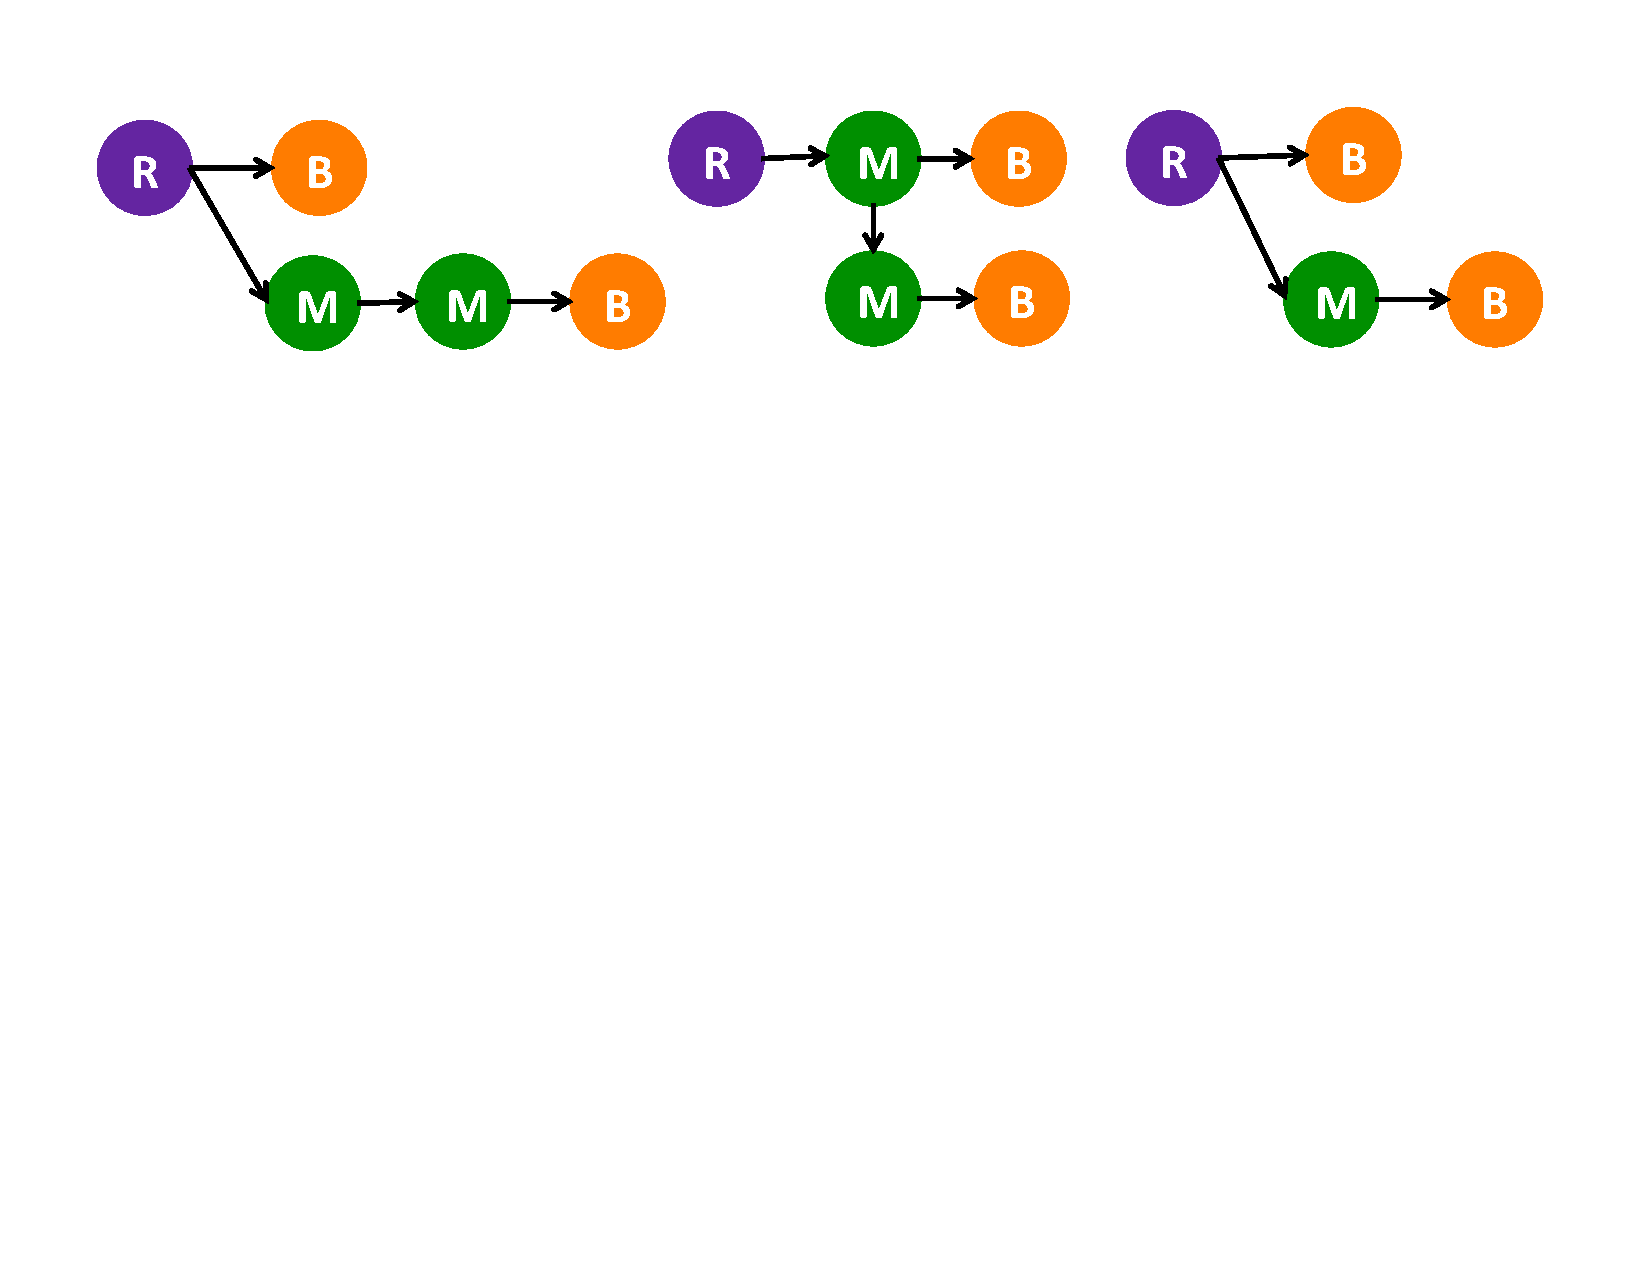
\includegraphics[trim={0 0 0 0}, clip, width=9cm]{Images/traces.pdf}}
	\caption{Interaction trace examples: (R) = Recommendation, (M) = Manual, (B) = Bookmark}
	\vspace{-10pt}
	\label{fig:traces}
\end{figure}

\stitle{3. \SeeDB provides a starting point for analyses}. 
To our knowledge, \SeeDB is the first tool to provide recommendations for supporting visual
analysis.
As a result, we were interested in how recommendations could fit into the analytical workflow.
While a participant's exact workflow was unique, we repeatedly found specific patterns in the
interaction traces of \SeeDB.
Figure \ref{fig:traces} shows examples of three such traces.
Interaction traces show that participants often started with a recommended visualization, 
examined it, modified it one or more times (e.g. by changing to a different aggregate function 
or measure attribute) and bookmarked the resulting visualization.
%  {\em recommendation 
% $\rightarrow$ manual\_modify $rightarrow$ manual\_modify $rightarrow$ \ldots bookmark}.
% Specifically, participants would often start from one of the recommendations and explore other
% visualizations that were variations of it (e.g. different aggregation or measure attribute) 
% until they found an interesting visualization.
% \mpv{can I put any data here?}
Thus, even if participants did not bookmark recommendations directly, their often created
small variations of the visualization and bookmarked them.
In other words, along with providing recommendations that were interesting by themselves, \SeeDB
helped direct participants to other interesting visualizations by {\em seeding} their analysis.
This pattern was highlighted in user comments as well; e.g.,
``\ldots would be incredibly useful in the initial analysis of the data'', 
``\ldots quickly deciding what correlations are relevant and gives a quick peek'',
``\ldots great tool for proposing a set of initial queries for a dataset''.
In addition to understand the role recommendations played in analysis, these observations 
also serve to reinforce the design choice of \SeeDB as a complement to a traditional
visualization system vs. a standalong system; the mixed-initiative nature of the tool 
is essential for it to be functional in visual analysis.
}


\techreport{
\subsection{Limitations}
Given that both studies described above were conducted in the lab, the studies had limitations.
First, due to constraints on time and resources, the sample sizes for both studies were small.
A larger set of participants and spread of datasets could be used to further demonstrate the
efficacy of our system.
Second, our user studies were conducted with graduate students participants who, on one hand, 
likely have higher data analysis skills than typical users, while on the other hand, are 
not experts in the dataset being analyzed.
Consequently, our results represent results the perspective of capable data analysts who 
have limited familiarity with the data.
We find that \SeeDB is particularly well suited for this particular setting of initial data 
analysis when the user is not very familiar with the data (\~ coldstart).
It would be instructive to evaluate \SeeDB on datasets about which users have expert knowledge.
Finally, we note that being a research prototype, limited functionality of \SeeDB (e.g. in types of
charts) and potential issues with learnability and interactivity may have also had an impact on
our study.

\mpv{Also: The datasets we evaluated had a relatively small (< 100) number of potential visualizations;
it would be valuable to evaluate the performance of \SeeDB on datasets with thousands of potential
visualizations.
It is also possible that some datasets were easier to interpret than others.
}
}



% 86\% of participants indicated that the recommendations sped up their analysis.


% When asked to rate the recommendations provided by \SeeDB, 78\% participants indicated that the
% recommendations were either ``Helpful'' or ``Very Helpful''. 
% We also found that 90\% of participants found the comparative visualizations shown by \SeeDB 
% helpful in their analysis.
% 66\% of participants indicated that the recommendations needed improvement, in particular,
% participants were interested in seeing different types of charts (e.g. geographical, time series)
% and obtaining measures of statistical significance.

% \stitle{Qualitative Feedback}. In their qualitative feedback, participants highlighted the importance of 
% a tool like \SeeDB at the initial stages of analysis. 
% One partitipant said, {\em ``It's a great tool for proposing a set of initial queries for a dataset I have never seen. 
% And from these visualizationns, I can figure out which related patterns to dig into more.''}
% Others thought that the strength of the tool was in quickly finding relevant trends, {\em ``It's a good tool that helps 
% in quickly deciding what correlations are relevant and gives a quick peek''}. 
% Overall, participants indicated that \SeeDB was particularly suited for exploratory analysis of new datasets, 
% {\em ``I thought SeeDB was very helpful in helping me get more familiar with a new dataset quickly.''}.



